\chapter{Body of my thesis}
\label{chapter:body}
\thispagestyle{myheadings}

% set this to the location of the figures for this chapter. it may
% also want to be ../Figures/2_Body/ or something. make sure that
% it has a trailing directory separator (i.e., '/')!
\graphicspath{{2_Body/Figures/}}

\section{Some results}
\label{sec:results}

Here goes all the important stuff, likely with a lot of graphics like this:

\begin{figure}[htb]
  \begin{minipage}[t]{0.49\linewidth}\centering
    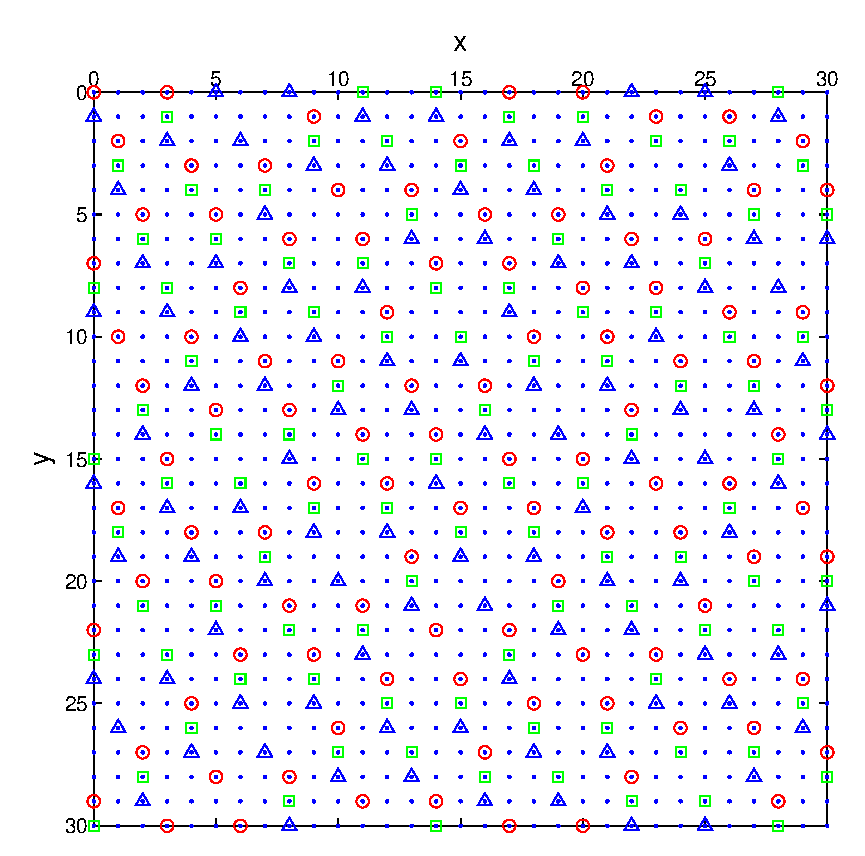
\includegraphics[width=7cm]{figure_sampling_view1.eps}
    \medskip
    \centerline{(a)}
  \end{minipage}\hfill
  \begin{minipage}[t]{0.49\linewidth}\centering
    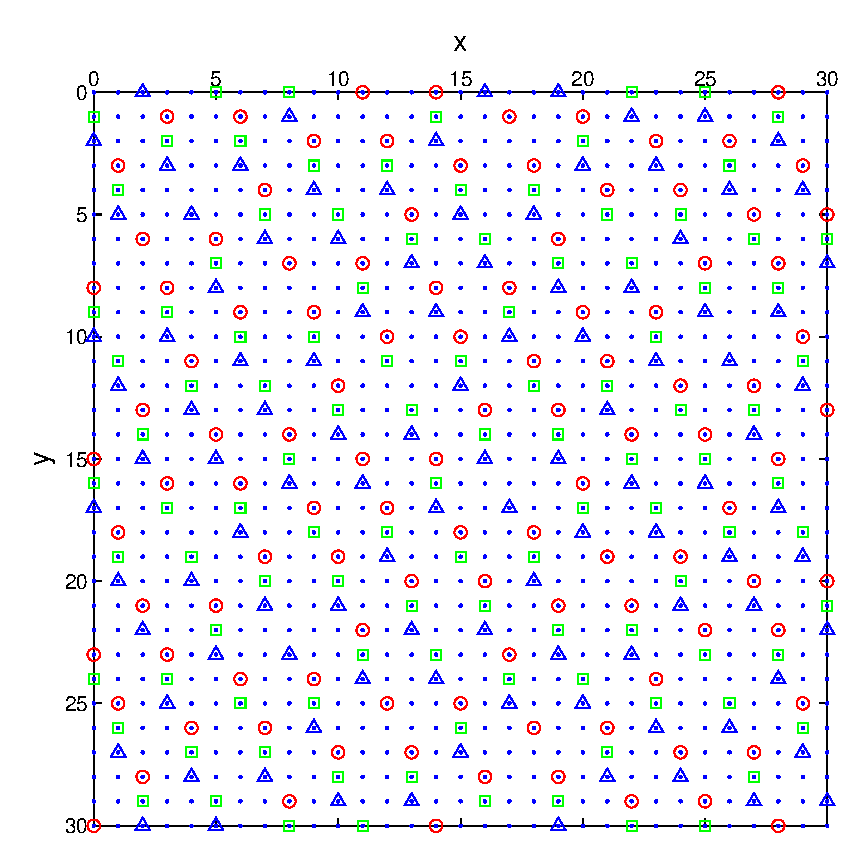
\includegraphics[width=7cm]{figure_sampling_view2.eps}
    \medskip
    \centerline{(b)}
  \end{minipage}
  \caption{Assignment of single-view intensities to RGB components: (a) view
    \#1; and (b) view \#2. }
  \label{fig:Sampling}
\end{figure}

In all likelihood, you will need to insert tables. See one example on the next page.
\clearpage

\begin{table}[h]
	\caption{Absolute disparity error per pixel for the test data from
		Fig.~\ref{fig:Sampling} and different parameter values. In each experiment one
		parameter is adjusted while other parameters are unchanged.} 
	\centering
	\renewcommand{\arraystretch}{1.2}
	\begin{minipage}[b]{0.30\linewidth}
		\centerline{$\eta=6000$, $\mu=2000$}\smallskip
		\centering
		\begin{tabular}{ccc}
			\hline
			$K$ & $u_1$ & $u_2$\\
			\hline
			3   & 0.52 &0.46\\
			7   & 0.47 &0.43\\
			10  & 0.35 &0.36\\
			12  & 0.37 &0.36\\
			\hline
		\end{tabular}
	\end{minipage}
	%
	\begin{minipage}[b]{0.34\linewidth}
		\centerline{$K=10$, $\mu=2000$}\smallskip
		\centering
		\begin{tabular}{ccc}
			\hline
			$\eta$ & $u_1$ & $u_2$\\
			\hline
			1000&0.54& 0.45\\
			3000&0.43& 0.40\\
			6000&0.35& 0.36\\
			9000&0.37& 0.37\\
			\hline
		\end{tabular}
	\end{minipage}
	%
	\begin{minipage}[b]{0.32\linewidth}
		\centerline{$K=10$, $\eta=6000$}\smallskip
		\centering
		\begin{tabular}{ccc}
			\hline
			$\mu$ & $u_1$ & $u_2$\\
			\hline
			100 &1.00&1.16\\
			1000&0.53&0.47\\
			2000&0.35&0.36\\
			3000&0.44&0.43\\
			\hline
		\end{tabular}
	\end{minipage}
	%
	\label{tab:Parameters}
\end{table}

Of course, there must be a Table of Contents, List of Figures and List of Tables at the beginning of the thesis, but this is all set up automatically.

{\bf Important}: You will also be using a lot of citations. The format in this template follows the so-called APA style and looks as follows in the document body: \cite{lamport1985:latex}, \cite{Debr01}. There are no numbers in the list of references -- the list is sorted alphabetically according to the first author's last name.

Other styles of references are allowed by the library as well, e.g., ``plain'' or ``'ieee'', which use numbers in square brackets both in the document body and in the list of references. In order to use another style of references, e.g., ``plain'', follow the steps below:
%
\begin{enumerate}
  \item In ``thesis.tex'' file:
	\begin{itemize}
	  \item comment out the line ``$\backslash$usepackage\{apalike\}'' at the top of the file,
	  \item replace ``$\backslash$bibliographystyle\{apalike\}'' with ``$\backslash$bibliographystyle\{plain\}'' towards the bottom of the file.
	\end{itemize}
  \item In ``bu\_ece\_thesis.tex'' file, comment out all lines in the BIBLIOGRPAHY section (lines 503-517) and save it!
  \item Recompile ``thesis.tex'' twice
\end{enumerate}

